\setaachaptext[45]{this appendix present the rationale behind the names}
\chapter{Etymology}
\label{a:etymology}

\section{\Starburst}

\begin{quote}\itshape%
	In astronomy, \emph{starburst} is a generic term to describe a region of space with an abnormally high rate of star formation.
	It is reserved for truly unusual objects.%
	\footnote{Lemma `Starburst region' of Wikipedia, October 2013}
\end{quote}


\Starburst* is used as the name of the many-core architecture in this thesis, but the project also includes numerous scripts to automatically generate a complete \ac{SoC} from a single architecture input file.
Therefore, this project is more or less a starburst in embedded systems, because of the easy and quick method of creating new flavors of many-core \acp{SoC}, complete with network configuration, \ac{OS} and bootstrap code.

At the moment, the project contains around \num{59000} lines of C/C++ code, \num{14000} lines of \noac{VHDL}, \num{5000} lines of Makefiles, and \num{3000} lines of other sources, including assembly, Haskell and \thecmd{gawk}.
In comparison, this thesis consists of around \num{12500} lines of \LaTeX.

A real starburst is cluster \noac{NGC}~3603, as depicted by \vref{fig:ety:starburst}\footnote{\url{http://hubblesite.org/gallery/album/pr2007034b/}}.
The cover image of this thesis is the star-forming region \noac{LH}~95 in the Large Magellanic Cloud\footnote{\url{http://hubblesite.org/gallery/album/pr2006055a/}}.
Although this is an active region, it is not classified as a starburst.

\begin{figure}%
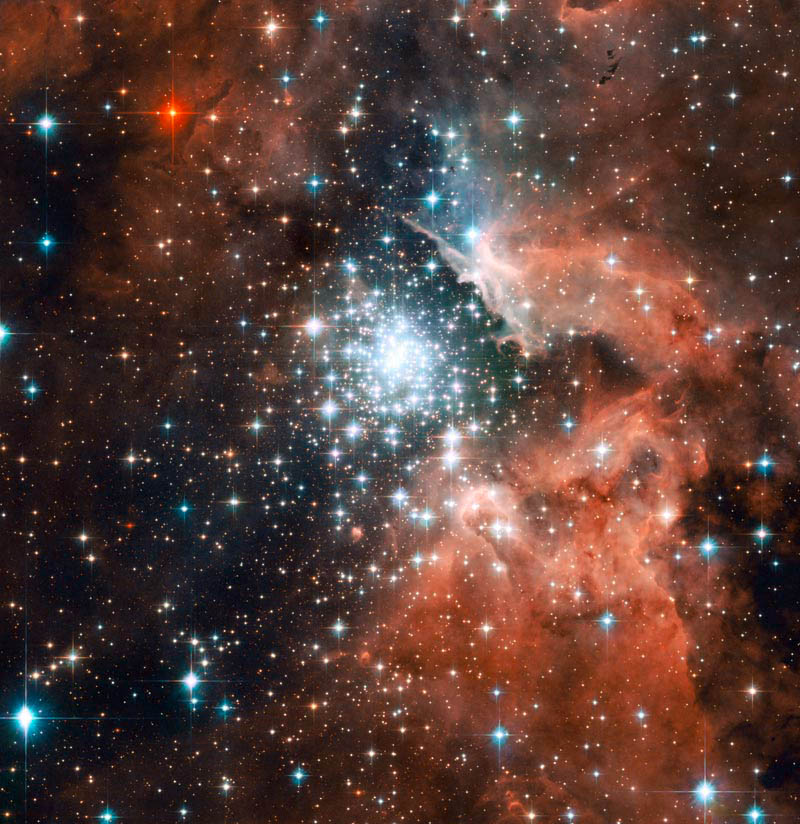
\includegraphics[width=.7\linewidth]{figures/ety_starburst}%
\caption{Starburst in cluster \noac{NGC}~3603}%
\label{fig:ety:starburst}%
\end{figure}


\section{\Warpfield}

The Alcubierre warp drive metric is a theoretic propulsion engine, which generates a field or `bubble' of expansion and contraction of space around the spacecraft.
Even though general relativity allows this type of propulsion, and it is a successful method in science-fiction series, any practical implementations is not expected soon%
\footnote{H.\ White. \href{http://ntrs.nasa.gov/archive/nasa/casi.ntrs.nasa.gov/20110015936_2011016932.pdf}{\textit{Warp Field Mechanics 101}}, NASA, 2011.}.
As the \Warpfield* \ac{NoC} targets high transmission speed, like most \acp{NoC} do, such a name seems appropriate for a subsystem of \Starburst.


\section{\Helix}

The operating system running on the \MicroBlazes, called \Helix*, is named after the Helix Nebula (\noac{NGC}~7293).
Its appearance (see \vref{fig:ety:helix}\footnote{\url{http://hubblesite.org/gallery/album/pr2004032d/}}) explains its nick name: Eye of God.
Mostly because of this name, it is appropriate to use it as the name of an \ac{OS}.

\begin{figure}%
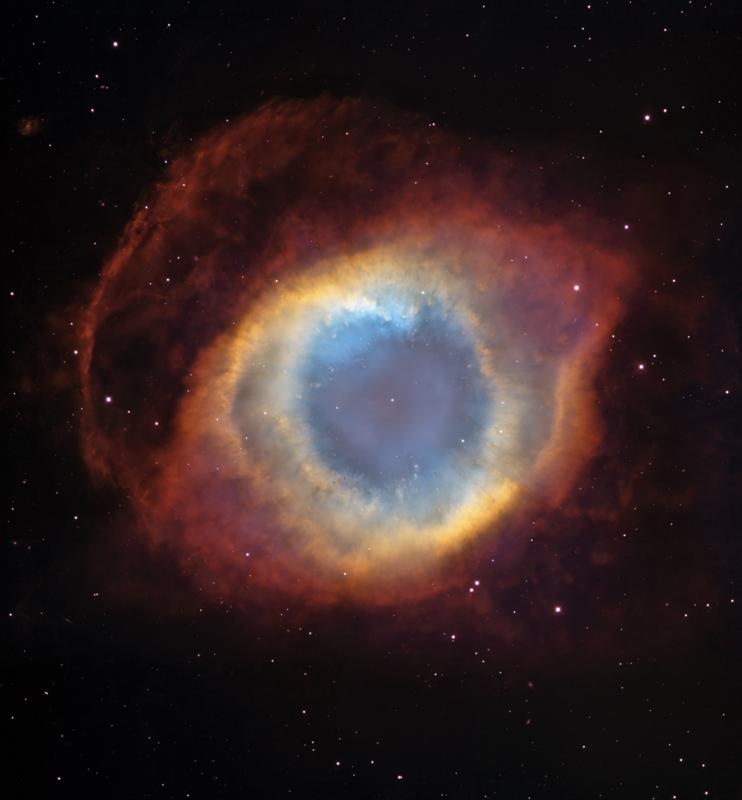
\includegraphics[width=.7\linewidth]{figures/ety_helix}%
\caption{Helix Nebula}%
\label{fig:ety:helix}%
\end{figure}


\section{\theapp{skat}}

Programs running on \Starburst, under supervision of \Helix, have the name \theapp*{skat} by default, just as \thecmd{gcc} produces \theapp{a.out} by default.
The name stems from the star Skat, or Delta Aquarii.
This star is part of the constellation Aquarius---the same constellation the Helix Nebula is located in.
Therefore, \Helix watches over \theapp{skat}.

\section{\ourfp}

If one reads the ++ as being an N, the name of the functional language in C++ coincides with Lambda Cen(tauri) Nebula.
\Vref{fig:ety:lambda}\footnote{\url{http://www.eso.org/public/images/eso1322a/}} shows a picture of this star cluster, which is also designated \noac{IC}~2944.
Dark dust clouds are presumed to play a role in the bright nearby star formation.
One can think of an analogy between this relation, and that of C++ and languages based on \lcalc.

\begin{figure}%
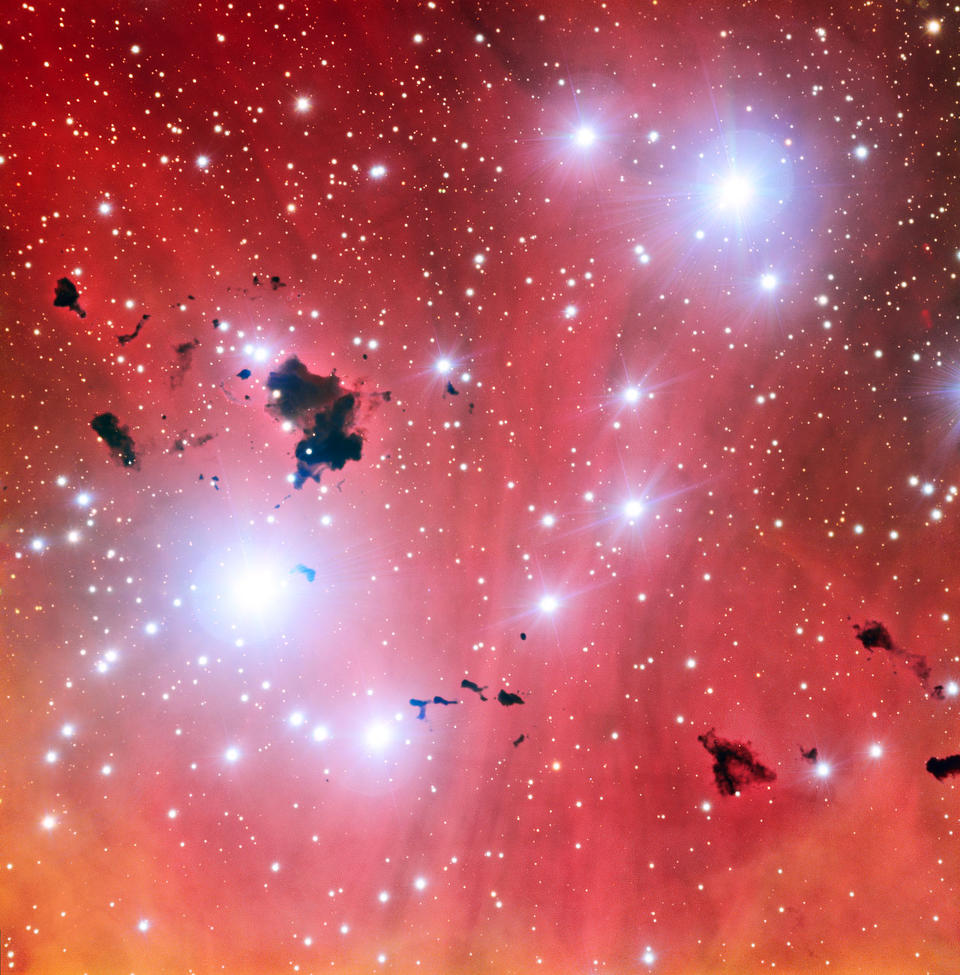
\includegraphics[width=.7\linewidth]{figures/ety_lambda}%
\caption{\noac{IC}~2944 cluster}%
\label{fig:ety:lambda}%
\end{figure}

